% Writeup for MDS
% David Lawrence Miller
% d.l.miller@bath.ac.uk
  
\documentclass[a4paper,10pt]{article}
\setlength{\textheight}{22.5cm}
\setlength{\textwidth}{6.47in}
\setlength{\oddsidemargin}{-1mm}
\setlength{\topmargin}{0.1cm}
\setlength{\evensidemargin}{-5mm} 
 
% Load some packages
\usepackage{times, amsmath, amssymb, amsfonts, url, natbib, bm, rotating}
 
\usepackage{multirow}
\usepackage{graphicx}

% top matter
\title{Multidimensional scaling as a tool for smoothing over complex regions}
\author{David Lawrence Miller\\Mathematical Sciences\\University of Bath\\\texttt{d.l.miller@bath.ac.uk}}
 
% Shortcuts
% Probability
\newcommand{\prob}[1]{\mathbb{P}\left[ #1 \right]}
% Schwarz-Christoffel
\newcommand{\sch}{Schwarz-Christoffel }
% fprime
\newcommand{\fprime}{f^\prime(z)}
% figure reference command
\newcommand{\fig}[1]{\emph{fig.} (\ref{#1})}
% Figure reference command
\newcommand{\Fig}[1]{\emph{Fig.} (\ref{#1})}
% equation reference command
\newcommand{\eqn}[1]{\emph{eqn.} (\ref{#1})}
% phi inverse
\newcommand{\phiinv}{\phi^{-1}}
% use other phi
\renewcommand{\phi}{\varphi}
%transpose
\newcommand{\tr}[1]{#1^{\text{T}}}
% diagonal
\newcommand{\diag}{\text{diag}}
% call \times \cross
\newcommand{\cross}{\times}


\begin{document}
 
% The abstract
%\begin{abstract}
%Here.
%\end{abstract}
 
 
% New theorem for theorems
\newtheorem{thm}{Theorem}[section]
 
%New theorem for definitions
\newtheorem{defn}{Definition}[section]
 
\maketitle

%\markright{TECH. DETAILS OF SCHWARZ-CHRISTOFFEL MAPPING}

\section{Introduction}

Multidimensional scaling (MDS) or, as it is often referred to, principle coordinates (PCO) is a method commonly used in multivariate analysis to find a new configuration of the data based on the distances between the points (\cite{chatfieldcollins}, p. 187.) In this new configuration, the Euclidean inter-point distances are approximately the same as their distances in the original data. Most often, MDS is used as a dimension reduction technique, finding a projection of data into lower dimensional space, while still retaining information about the distances between the points. It is closely related to techniques such as PCA (\cite{chatfieldcollins}, p. 200) and canonical correspondence analysis (\cite{terbraak}.)

Multidimensional scaling offers an obvious framework for the problem of smoothing over a region with a complex boundary. We can use the within-area distances to configure the points such that the distances between the points are (approximately) preserved.

The modelling strategy is as follows:

\begin{enumerate}
\item Take a regular grid over the domain and perform MDS on this.
\item Using this grid, insert the sample points into this configuration.
\item Fit the smooth to the MDS configuration of points.
\item Depending on the inference needing to be done, the points can be back-transformed.
\item If prediction is required, take those predicted points and insert them into the MDS configuration, predict using the smooth and then back-transform to the original space.
\end{enumerate}

The back-transform above is trivial if an index of the points is kept. The reasoning behind this strategy will be explained below.

The rest of this report is structured as follows: in section (2) an overview of MDS is given, along with technical details of how the MDS configuration is calculated; section (3) focuses on how the within-area distances are found; section (4) shows the some examples of this method on simulated data. I conclude with a proposed course of action to improve the method.

\section{Multidimensional Scaling}

The basic concept behind MDS is to take the data, calculate their inter-point distances and then find a new coordinate system based on those inter-point distances. We do this by simply performing an eigen-decomposition on the matrix of distances between points.

\subsection{Finding the new point configuration}

We first define $d_{ij}$ as the distance between the points $i$ and $j$. These form a (symmetric) matrix, $D$, with $ij^{\text{th}}$ element $d^2_{ij}$. In our case, we would like $d_{ij}$ to be the shortest distance between the points, given the path between the points remains within the domain. Finding $d_{ij}$ is discussed in the next section, for the moment let us assume that $D$ is known and gives the shortest within-domain distance between points.

\cite{diaconis08} gives a clear definition of the algorithm (due to \cite{schoenberg35}) for finding the new locations of points given we know the $d_{ij}$s. 

First, take the unknown new locations and putting them in an $n \times p$ matrix, $\tilde{X}$. Let $S=\tilde{X}\tr{\tilde{X}}$; performing an eigen-decomposition we can see that $S=U\Lambda\tr{U}$. We may then represent $S$ in some arbitrary number of dimensions, $k$, by picking the $k$ largest eigenvalues of $S$. In a multivariate analysis we usually want $k<p$ to reduce the dimensionality of the problem, although that is not the case here, so we choose $k=p$.

We are interested in

\begin{equation}
\tilde{X}=U\Lambda^{\frac{1}{2}}.
\end{equation}

We can relate $D$ to $S$ by first defining:

\begin{equation}
H = I-\frac{1}{n}\mathbf{1}\tr{\mathbf{1}}.
\end{equation}

By pre- and post-multiplying any matrix by $H$ we double centre it (such that row and column means are 0.) We then obtain:

\begin{equation}
S = -\frac{1}{2}HDH.
\end{equation}

See \cite{diaconis08} for a simple proof of this.

So, in order to obtain a the new configuration of points using MDS (given that we have some set of inter-point distances) we merely need to double centre the matrix of distances and perform an eigen-decomposition.

Multidimensional scaling may be performed in \textsf{R} using the \texttt{cmdscale} function. 

\subsection{Gower's interpolation} 

It is likely that we may be in a position where the coordinate system has been found by MDS but we need to insert further points into our MDS representation; for example when further data is collected, or in order to predict over points not in the sample. In this case we would like to insert those new points into the configuration given by MDS. A number of methods have been developed over the past 40 years. Gower's interpolation (\cite{gower1968}) is covered here.

Gower's method relies on taking a single new point $x_{\text{new}}$, and inserting it into a new (orthogonal) dimension in the configuration. It is positioned at a distance from the MDS points ($\tilde{X}$) which is approximately the same as the distance between $x_{\text{new}}$ and the points in Euclidean space. The extra dimension is then projected on to the old axes. The technical details of the computation are detailed first, followed by some problems arising from the use of this method. 

\subsubsection{Gower's interpolation formula}

We may find the new position, $\tilde{x}_{\text{new}}$, of some new datum $x_{\text{new}}$ using:

\begin{equation}
\tilde{x}_{\text{new}} = \frac{1}{2} \Lambda^{-1} \tr{\tilde{X}} \mathbf{d},
\label{gower}
\end{equation}

here $\Lambda$ ($k \cross k$) and $\tr{\tilde{X}}$ ($k \cross n$) are as above, $\mathbf{d}$ ($n \cross 1$) is defined as the squared distance between $x_{\text{new}}$ and the points in $\tilde{X}$.


\subsubsection{Problems arising}

If our sample is not representative of the whole of the domain, the eigenvalues in $\Lambda$ may not represent the space correctly and, as such, we may then insert the point(s) incorrectly. This could happen if the sample is taken from only half of the space or, more pathologically, there were a trend in the sample locations, in this case only a portion of the full information about the domain would be included in the model. This would lead to the incorrect eigenvalues being calculated. When Euclidean distances are used to calculate $D$ the eigenvalues are found correctly given that there is one more point than there are dimensions in the space (\cite{landmark},) provided that the points are not collinear. However, it is not clear what this criteria would be for the shortest paths used here. This problem can be rectified by using an appropriately spaced grid on the domain to calculate the eigen-decomposition, thus ensuring that the whole area is covered.

In the course of the projection onto the original MDS axes, we lose one of the coordinates (effectively truncating a dimension.) If the MDS axes were in two dimensions, it is possible that the point was not supposed to lie in the plane but rather this an extra dimension and its distance was truncated. This can cause distortions in the point configuration. An example of this is illustrated in \fig{bojinsert}. A more complete explanation and characterisation of this problem is given in \cite{Boj2009}. 

% diagram from Boj et al. 2009
\begin{figure}
\centering
% trim order l b r t
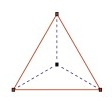
\includegraphics{figs/boj0.jpg} 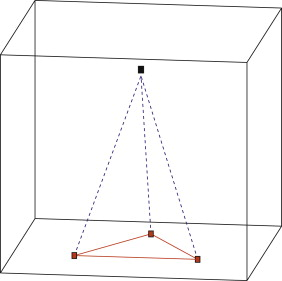
\includegraphics[width=1in]{figs/boj1.jpg} \\
\caption{Given the three points that make up the equilateral triangle in the left panel, if a new point is introduced then it will be mapped into a dimension orthogonal to that of the original points. This extra dimension is then truncated and the projection onto the plane used. Taken from \cite{Boj2009}.}
\label{bojinsert}
\end{figure}

The above distortion is compounded when extra points are added to the MDS configuration in an ``online'' manner. For example, say MDS has been performed on some set of points and then mapped them into the plane. Then suppose that new points are added into this configuration using Gower's interpolation. When the first point is added, say there is some error in its projection onto the plane from a third dimension, orthogonal to the first two. The second has the same problem, but now the second's position is calculated with respect to the first's (potentially incorrect) position too. The third is then calculated using the first and second and so on. This can be observed in \fig{gowererror}, where the red points should correspond to the gaps in the grid of black points, and the whole configuration should be identical to that of \fig{wt2dia} panel 2. It is for this reason that we do not insert the points online, but rather simultaneously insert all points.

% online insertion error in Gower
\begin{figure}
\centering
% trim order l b r t
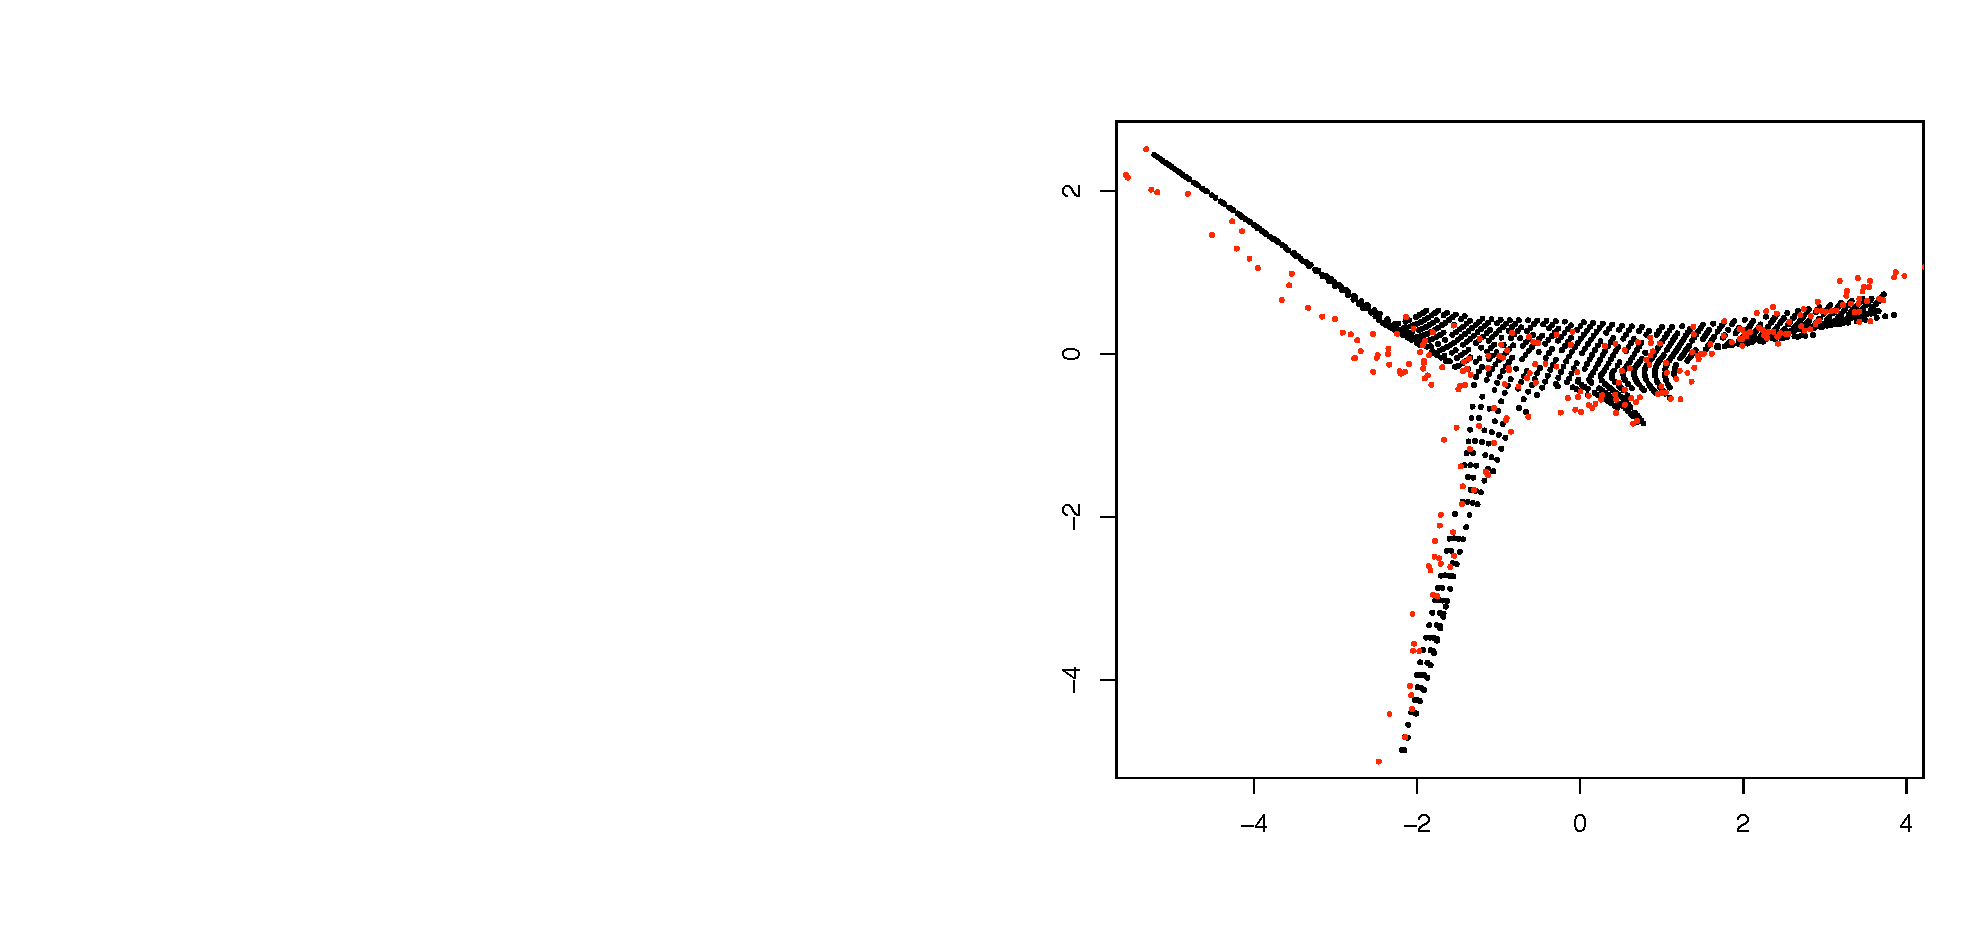
\includegraphics[width=4in]{figs/gowererror.pdf} \\
\caption{MDS configuration for the domain in \fig{wt2dia}. Black points are formed by the initial eigen-decomposition, where as the red points are positioned using Gower's interpolation online. The red points should be positioned in the ``holes'' in the black grid.}
\label{gowererror}
\end{figure}


Following from this, it is important to make sure that the MDS space is smooth in the sense that a grid of straight lines over the domain is mapped to a series of smooth lines. Taking the evenly spaced grid in \fig{wt2-grid-orig}, first MDS is performed on a dense point set of size 1253, and then a less dense grid is inserted using the method of Gower. The grid produced under the insertion can be seen in \fig{wt2-grid-full}. Taking a sample of 250 points from the 1253, an MDS configuration was also found and the same grid inserted (see \fig{wt2-grid-samp}.) From this it is clear that those points mapped into the domain are smooth but in the sample case the features in the far right of the shape (the less pronounced peninsulae) are squashed down.



% grid to map
\begin{figure}
\centering
% trim order l b r t
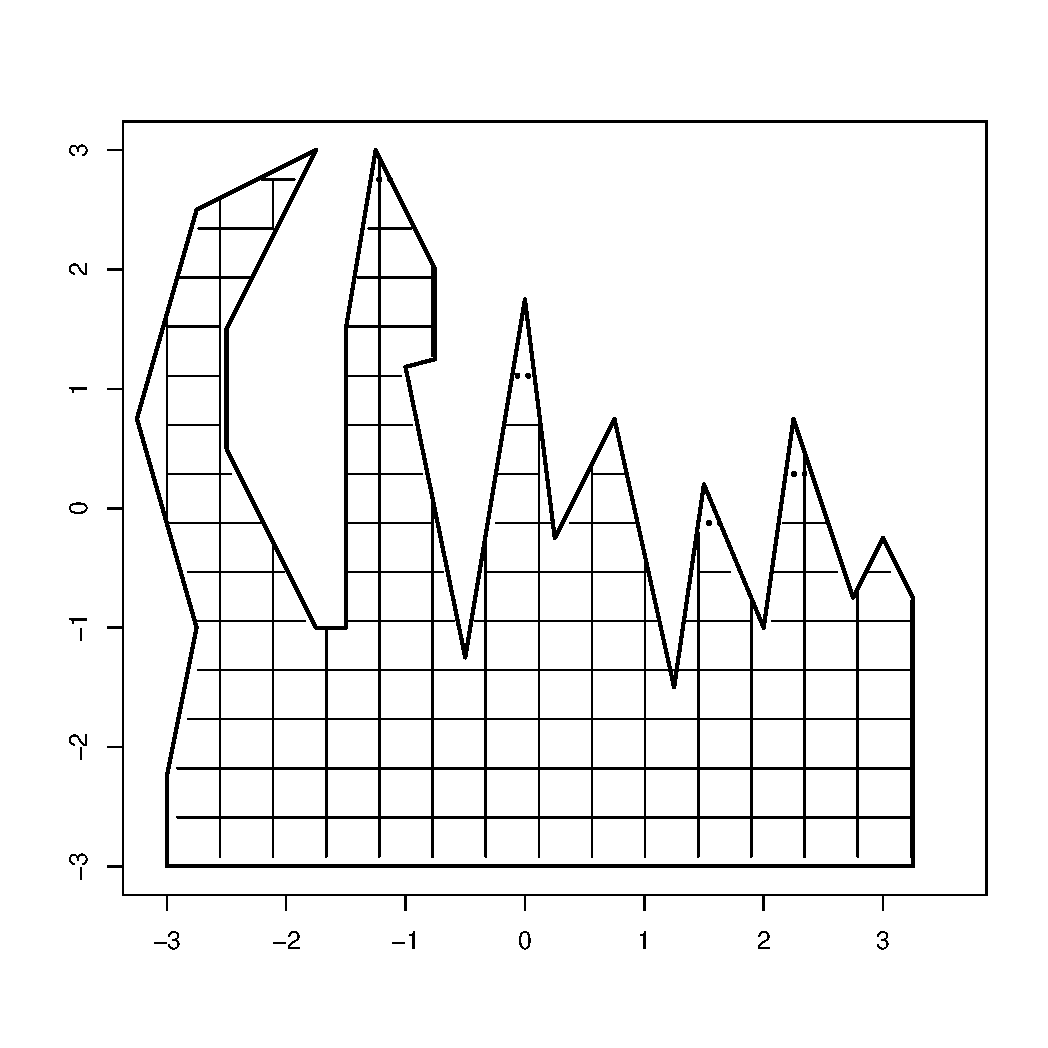
\includegraphics[width=4in]{figs/wt2-grid-orig.pdf} \\
\caption{The grid to be inserted into the MDS configuration.}
\label{wt2-grid-orig}
% generated using wt2-grid.R
\end{figure}

Given that the grid over the transformed space is smooth, how do the ``errors'' that can be seen in \fig{gowerfullinsert} occur? It turns out that although insertions using Gower's method are self-consistent, they are not consistent with the original MDS space. The following example shows that re-inserting points does not recover their MDS coordinates, but that the shape and distances are preserved.

% mapped grid (full)
\begin{figure}
\centering
% trim order l b r t
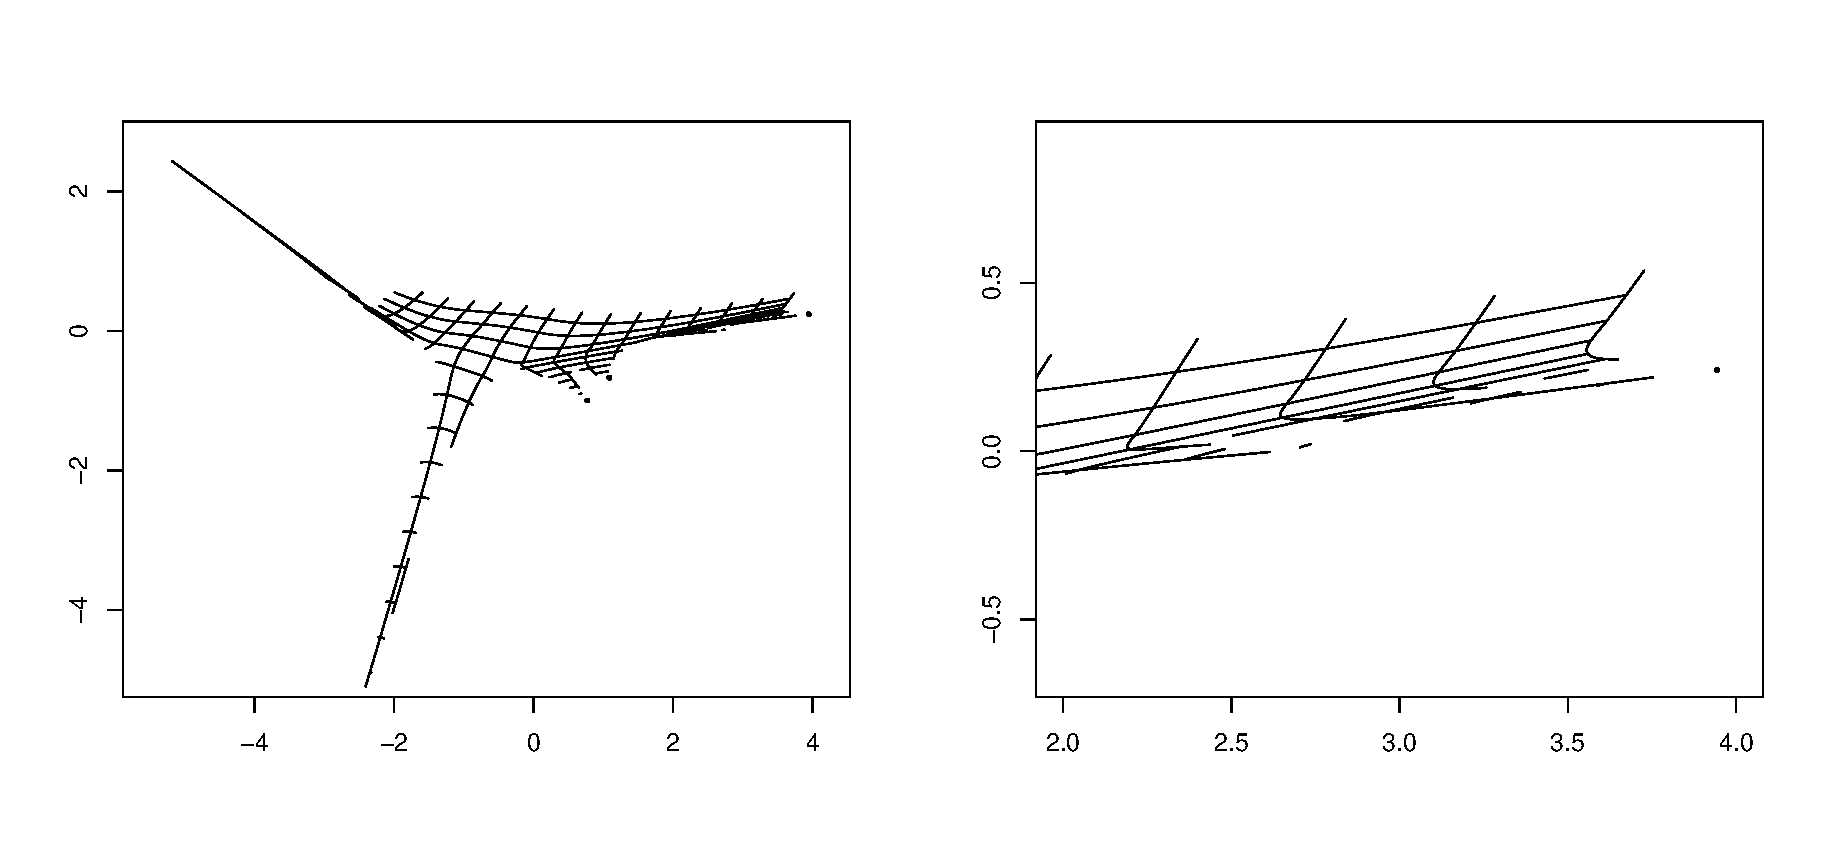
\includegraphics[width=5in]{figs/wt2-grid-full.pdf} \\
\caption{Inserted grid when 1253 points are used to create the initial MDS configuration. The right panel shows a zoom of the far right part of the configuration.}
\label{wt2-grid-full}
% generated using wt2-grid.R
\end{figure}

% mapped grid (samp)
\begin{figure}
\centering
% trim order l b r t
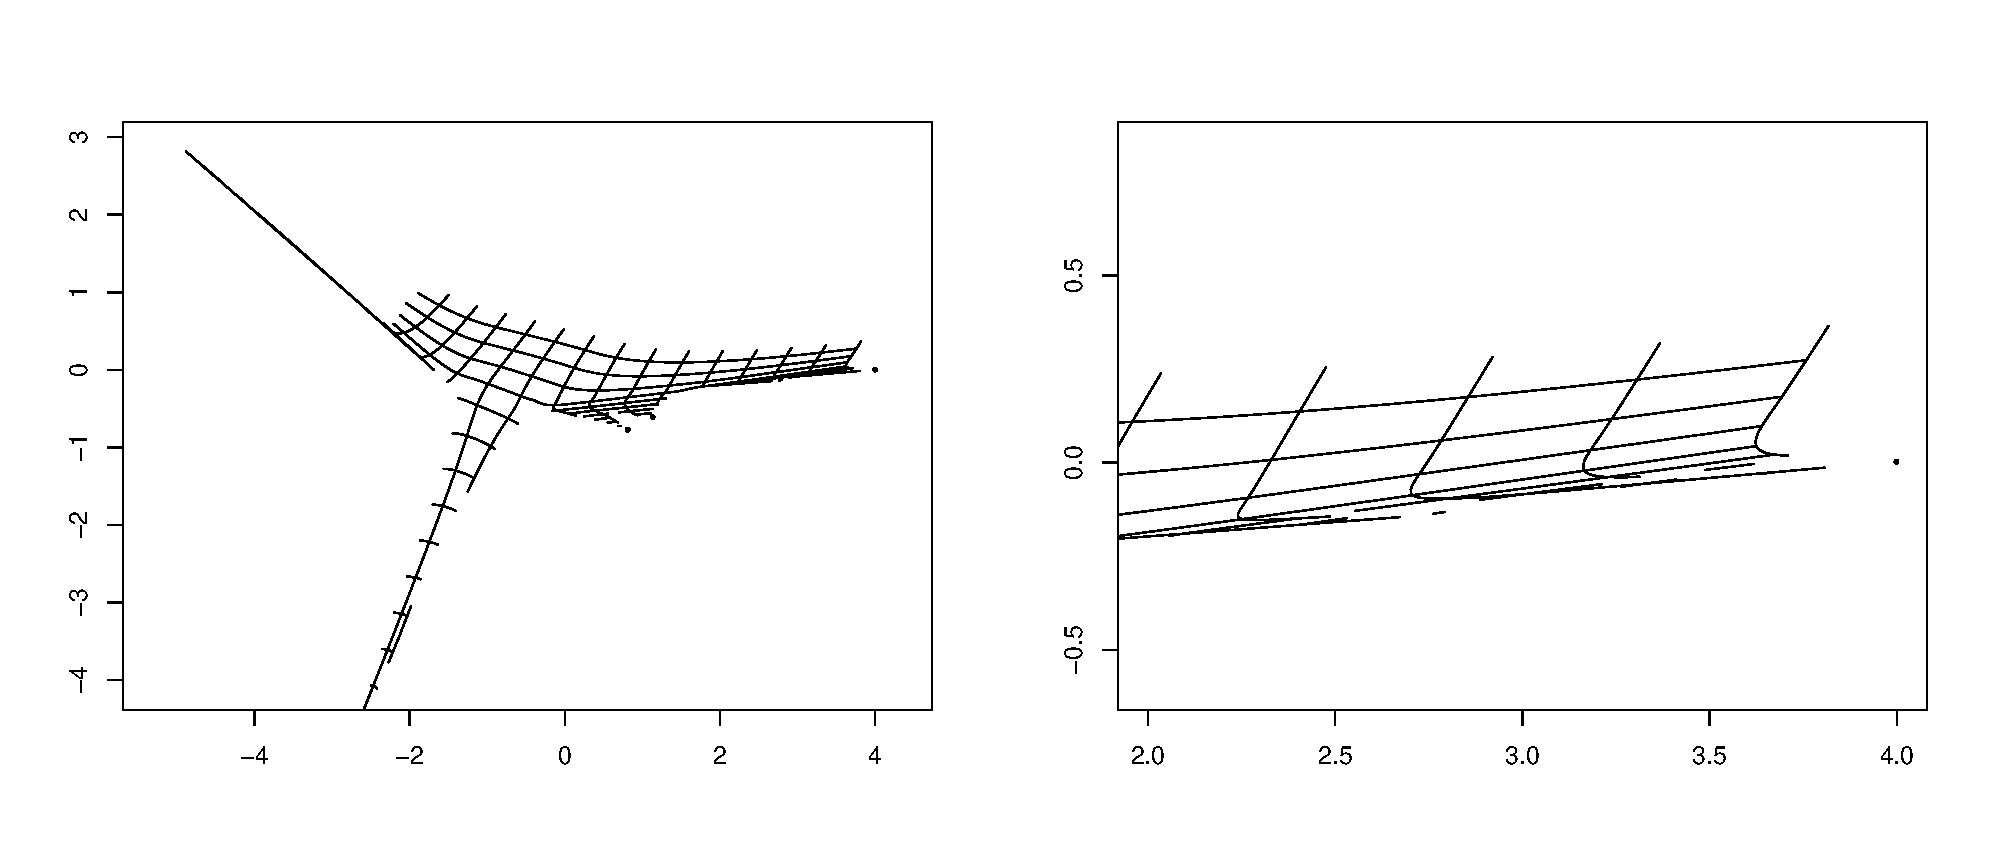
\includegraphics[width=5in]{figs/wt2-grid-samp.pdf} \\
\caption{Inserted grid when 250 randomly chosen points are used to create the initial MDS configuration. The right panel shows a zoom of the far right part of the configuration. Comparing this to that of \fig{wt2-grid-full}, one can see that the right side features have been squashed together.}
\label{wt2-grid-samp}
% generated using wt2-grid.R
\end{figure}


\subsubsection{Consistency of interpolated points}

It is important to note that those points found by simultaneous insertion via Gower's method are self-consistent but not consistent with the MDS configuration used to generate the inserted set. The following example shows this.

Take three points, equidistant, 1 unit apart, they have the following (Euclidean) distance matrix:

\begin{equation*}
D_3 = \begin{pmatrix} 0 & 1& 1\\1 & 0 & 1\\ 1 & 1 & 0\end{pmatrix},
\end{equation*}

graphically: \fig{cexample}, top left pane.

We find the MDS representation of the points in the same manner as \cite{diaconis08}.

First, double centring the matrix (making row and column means zero):

\begin{equation*}
\begin{aligned}
S &= -\frac{1}{2} HD_3H\\
    &= \begin{pmatrix} 1/3 & -1/6 & -1/6\\-1/6 & 1/3 & -1/6\\ -1/6 & -1/6 & 1/3\end{pmatrix},
\end{aligned}
\end{equation*}

where $H=I-\frac{1}{n}\mathbf{1}\mathbf{1}^\text{T}$.

Now, performing an eigen-decomposition on $S$,

\begin{equation*}
S = U \Lambda U^\text{T},
\end{equation*}

we obtain:

\begin{equation*}
U = \begin{pmatrix} 
	0 & 0.8164 & -0.5773\\
	-0.7071 & -0.4082 & -0.5773\\ 
	0.7071 & -0.4082 & -0.5773
	\end{pmatrix},\qquad
\Lambda = \begin{pmatrix} 
	1/2 & 0 & 0\\
	0 & 1/2 & 0\\ 
	0 & 0 & 2.2\cross10^{-16}
\end{pmatrix}.
\end{equation*}

Finally finding $X$,

\begin{equation*}
X=U\Lambda^{\frac{1}{2}}= \begin{pmatrix} 
	0 & 0.5773 & -8\cross10^{-9}\\
	-0.5 & -0.2886 & -8\cross10^{-9}\\ 
	0.5 & -0.2886 & -8\cross10^{-9}
	\end{pmatrix}.
\end{equation*}

Discarding the last column, we obtain the MDS coordinates:

\begin{equation}
\begin{pmatrix} 
	0 & 0.5773\\
	-0.5 & -0.2887\\ 
	0.5 & -0.2887
	\end{pmatrix},
\label{origMDScoords}
\end{equation}

giving the representation seen in \fig{cexample}, top right pane.

% grid to map
\begin{figure}
\centering
% trim order l b r t
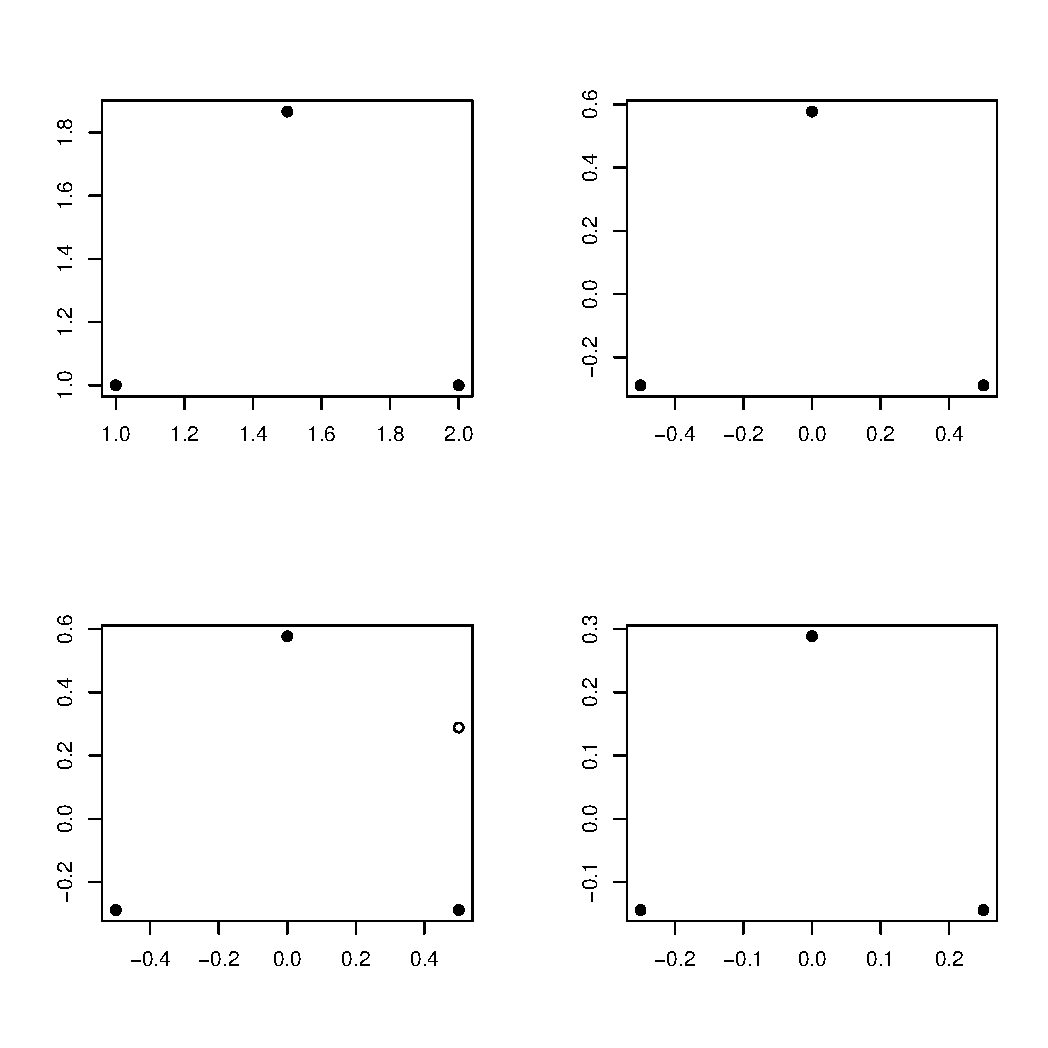
\includegraphics[width=3.5in]{figs/cexample-fig.pdf} \\
\caption{Example showing how the insertion of points is not consistent with previous point locations. Clockwise from top left: initial point configuration, MDS configuration of points, second point inserted and all points re-inserted.}
\label{cexample}
% generated using figs/cexample-figs.R 
\end{figure}

So, taking these points and re-inserting the second point into their MDS representation, we use equation (\ref{gower}). First, finding the vector of distances from point 2 to the other points in the non-MDS space:

\begin{equation*}
\mathbf{d}=\begin{pmatrix} 
	1\\
	0\\ 
	1
	\end{pmatrix},
\end{equation*}

and centring it to have mean zero:

\begin{equation*}
\mathbf{d}=\begin{pmatrix} 
	1/3\\
	-2/3\\ 
	1/3
	\end{pmatrix}.
\end{equation*}

And using Gower's formula:

\begin{equation*}
\begin{aligned}
\tilde{x}_{\text{new}} &= \frac{1}{2} \Lambda^{-1} \tr{\tilde{X}} \mathbf{d}\\
&=\begin{pmatrix}
0.5\\
0.2887\\
-2.4 \cross 10^{-9}\\
\end{pmatrix},
\end{aligned}
\end{equation*}

which is a reflection of the second point in equation (\ref{origMDScoords}). This can be seen in \fig{cexample}, bottom left pane.

Let us now see what happens when all three points are re-inserted. First generalise $\mathbf{d}$ to be a matrix, $\mathbb{D}$, giving the distances from the ``old'' points to our ``new'' points which double centred as above, by pre- and post-multiplying by the $H$ matrix. Now, equation (\ref{gower}) becomes:

\begin{equation*}
\tilde{X}_{\text{new}} = \frac{1}{2} \Lambda^{-1} \tr{\tilde{X}} \mathbb{D}\\
\end{equation*}

and so the coordinates obtained are:

\begin{equation*}
\tilde{X}_\text{new}=\begin{pmatrix}
-1.9\cross 10^{-17} & -0.25 & 0.25\\
 0.2887 & -0.1443 & -0.1443\\
-2.04\cross 10^{-9} &  1.2\cross 10^{-9} & 1.3\cross 10^-{9}\\
\end{pmatrix}
\end{equation*}

By analogy with the single point case, we take the transpose and remove the final column, thus obtaining:

\begin{equation*}
\begin{pmatrix}
-1.8\cross 10^{-17} &  0.2887\\
-0.25 & -0.1443\\
 0.25 & -0.1443\\
\end{pmatrix}
\end{equation*}

which are different from our original coordinates but, as can be seen from \fig{cexample}, bottom right pane, the distances and shape are preserved.

The above effect can be seen on a much larger scale in \fig{gowerfullinsert}. In this case 250 points were inserted simultaneously from the 1253 used to construct the MDS configuration. In this case we are inserting the same points as were in the original configuration again. Here the it can be seen that both sets of points are internally consistent but not consistent with each other.

% offline insertion error in Gower
\begin{figure}
\centering
% trim order l b r t
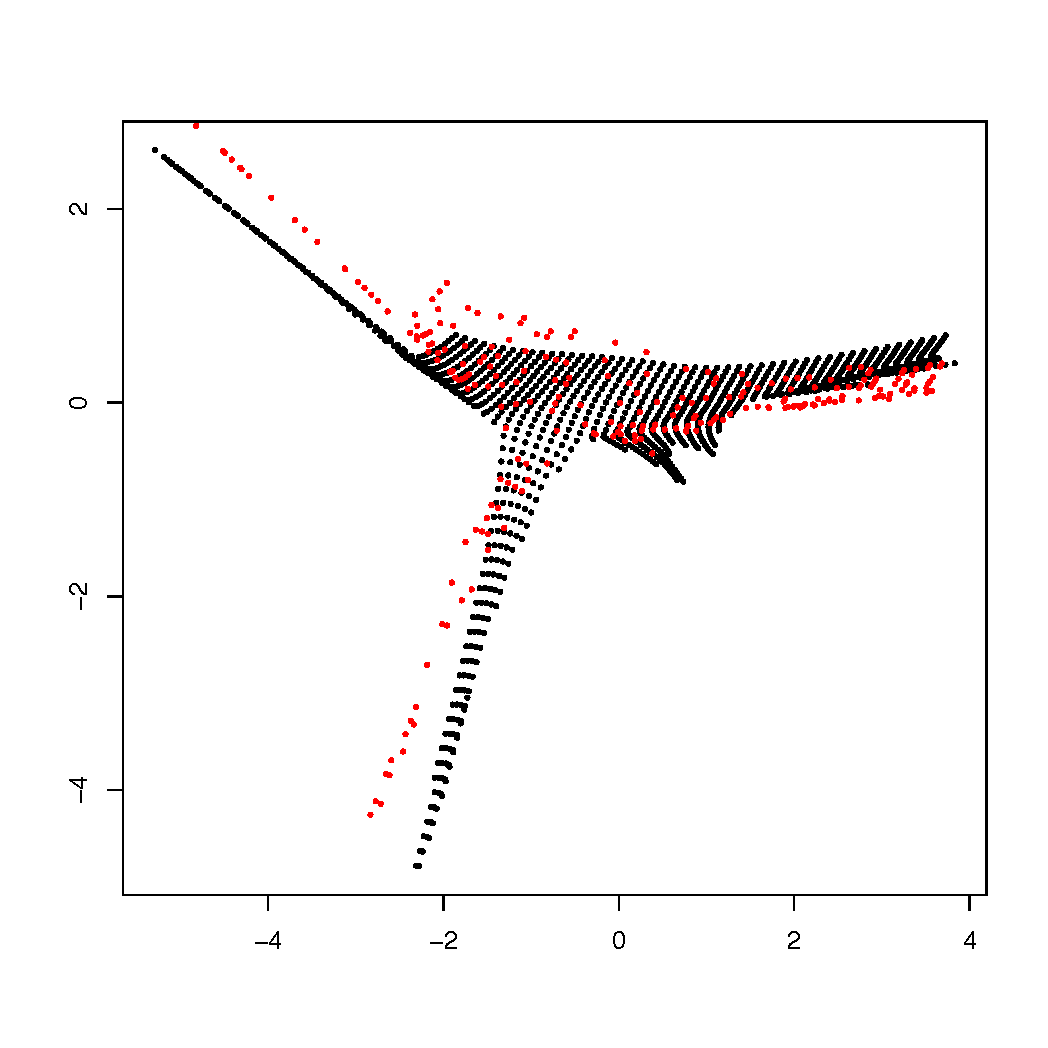
\includegraphics[width=4in]{figs/wt2-gowererr-fullover.pdf} \\
\caption{Error from inserting 250 points from the full MDS configuration back into the domain.}
\label{gowerfullinsert}
% generated (roughly) using wt2-insert-error.R
\end{figure}

It is for these reasons that we insert both the sample and the prediction from a regular grid.


\section{Finding the within-area distances}

The within-area distances to be fed to MDS are found using a novel algorithm. This works by tracing the edges of the polygon and then modifying the path by deleting and replacing portions of the path. 

Given that there is no direct path within the domain ($\Gamma$, say) between two points ($p_1$ and $p_2$, say), the algorithm proceeds as follows:

\begin{enumerate}
\item Draw a line between $p_1$ and $p_2$ (\fig{wdia}, ($i$)) and where they meet the boundary of $\Gamma$. Start the path as the lines from $p_1$, $p_2$ to their first intersection with the boundary of $\Gamma$. Then find the distance between these two intersection points in both directions, along the boundary (\fig{wdia}, ($ii$).) Choose the shorter of these add the paths between $p_1$, $p_2$ and the boundary and this is the starting path(\fig{wdia}, ($iii$).) 
\item Given a triple of vertices, ($v_i$, $v_{i+1}$, $v_{i+2}$) if the line between $v_i$ and $v_{i+2}$ is shorter than the path ($v_i$, $v_{i+1}$, $v_{i+2}$) and the line between $v_i$ and $v_{i+2}$ lies inside $\Gamma$ then delete $v_{i+1}$ (\fig{wdia}, ($iv$) and ($vi$).) This iterates over the entire path once, deleting all superfluous vertices. 
\item Given a triple of vertices, ($v_i$, $v_{i+1}$, $v_{i+2}$) if the path ($v_i$, some subset of the vertices of $\Gamma$, $v_{i+2}$) is shorter than the path ($v_i$, $v_{i+1}$, $v_{i+2}$) then replace $v_{i+1}$ with those elements of $\Gamma$ (\fig{wdia}, ($v$)). 
\item We then iterate between steps 2 and 3 until there has been no change from one run to the next (ie. convergence) or there have been too many iterations (\fig{wdia}, ($vi$).)
\end{enumerate}

% diagram for finding the shortest path in W
\begin{figure}
\centering
% trim order l b r t
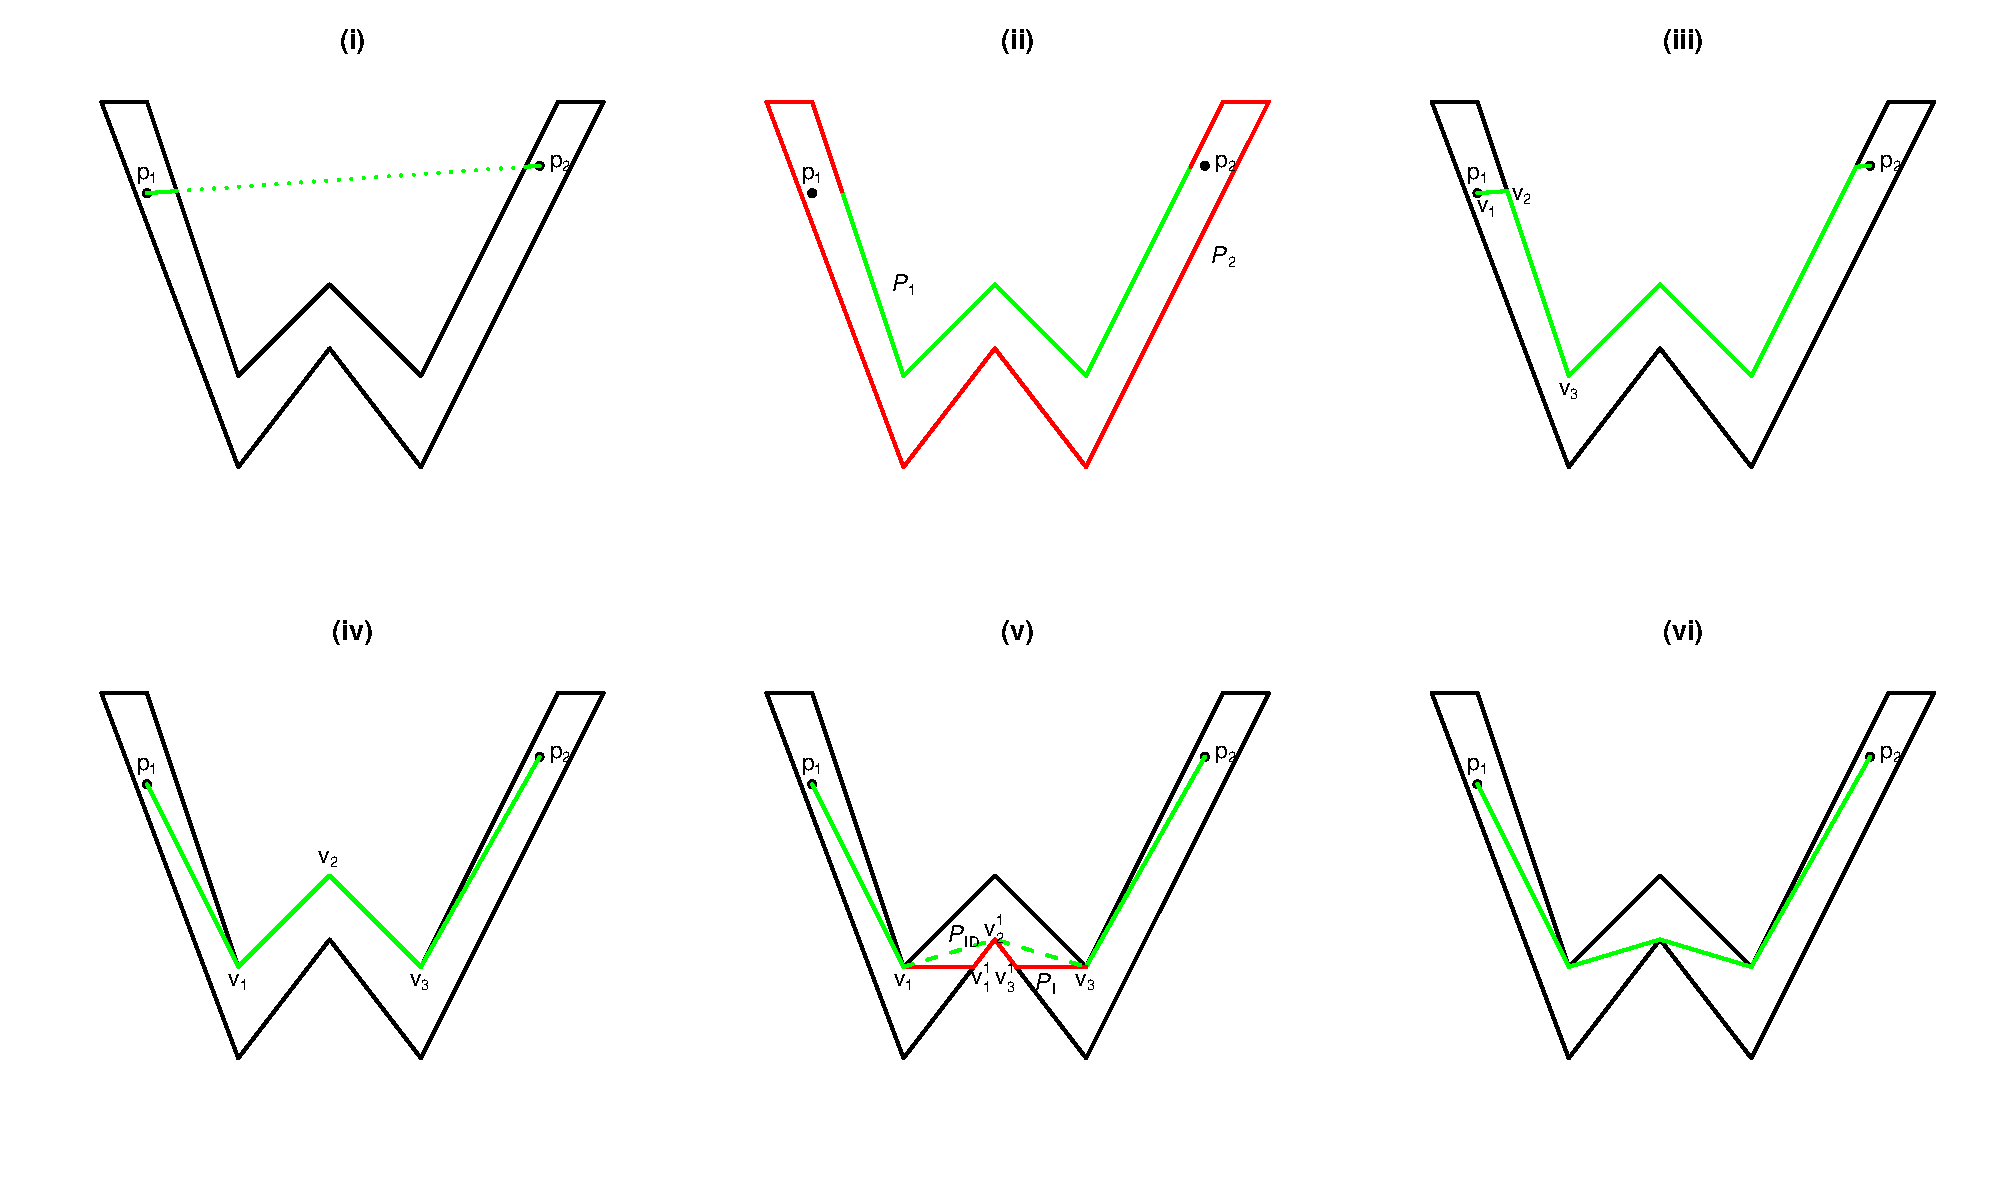
\includegraphics[trim=0in 0.5in 0in 0.25in, width=4in]{figs/wdia.pdf} \\
\caption{The green lines in ($i$) to ($vi$) show the path as the algorithm progresses from initial state to final, shortest path (bottom right.) }
\label{wdia}
% generate /phd-smoothing/mds-writeup/figs/distanceexplanation.R
\end{figure}


\section{Multidimensional scaling for complex domains}

Tying together the previous sections, we may now look at how, using MDS and our new algorithm, we can reconfigure the points in our domain.

\subsection{Ramsay's horseshoe}

\Fig{ramsay-mds} shows MDS being performed on the Ramsay horseshoe (\cite{ramsay}.) From this it is clear to see that performing MDS separates the two arms of the horseshoe.

% Ramsay MDSed 
\begin{figure}
\centering
% trim order l b r t
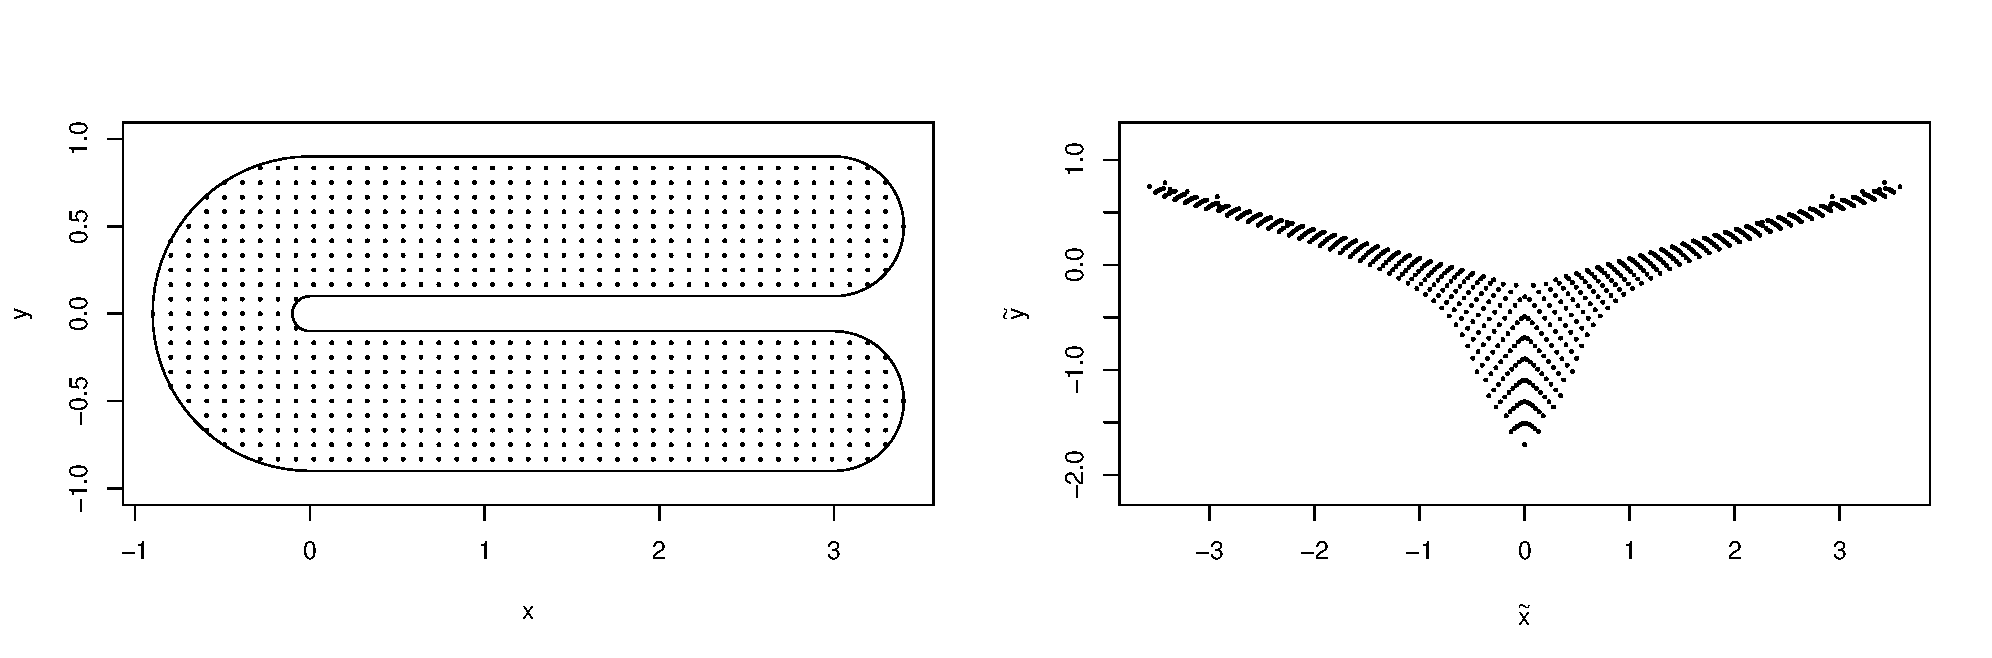
\includegraphics[trim=0in 0.5in 0in 0.25in, width=5.5in]{figs/ramsay-mds.pdf} \\
\caption{Left panel shows the horseshoe with 734 points. Right panel shows their configuration under MDS using the algorithm detailed above.}
\label{ramsay-mds}
% generate /phd-smoothing/mds-writeup/figs/ramsay-mds.R
\end{figure}

%An advantage of the MDS approach is that in our eigen-decomposition we may pick an arbitrary number of eigenvectors to retain and push the original set of points into higher dimensions. Using three eigenvectors we get the configuration in \fig{ramsay-mds-3d}.

The two eigenvalues returned from running \texttt{cmdscale} in \textsf{R} when we ask for a 2-dimensional representation are 2615 and 229. Adding another dimension gives a third eigenvalue of 46.8. Clearly significantly less variation is being explained in the third dimension, however this may well not be of primary concern if it prevents leakage.

% Ramsay MDS smooth fit (no noise)
\begin{figure}
\centering
% trim order l b r t
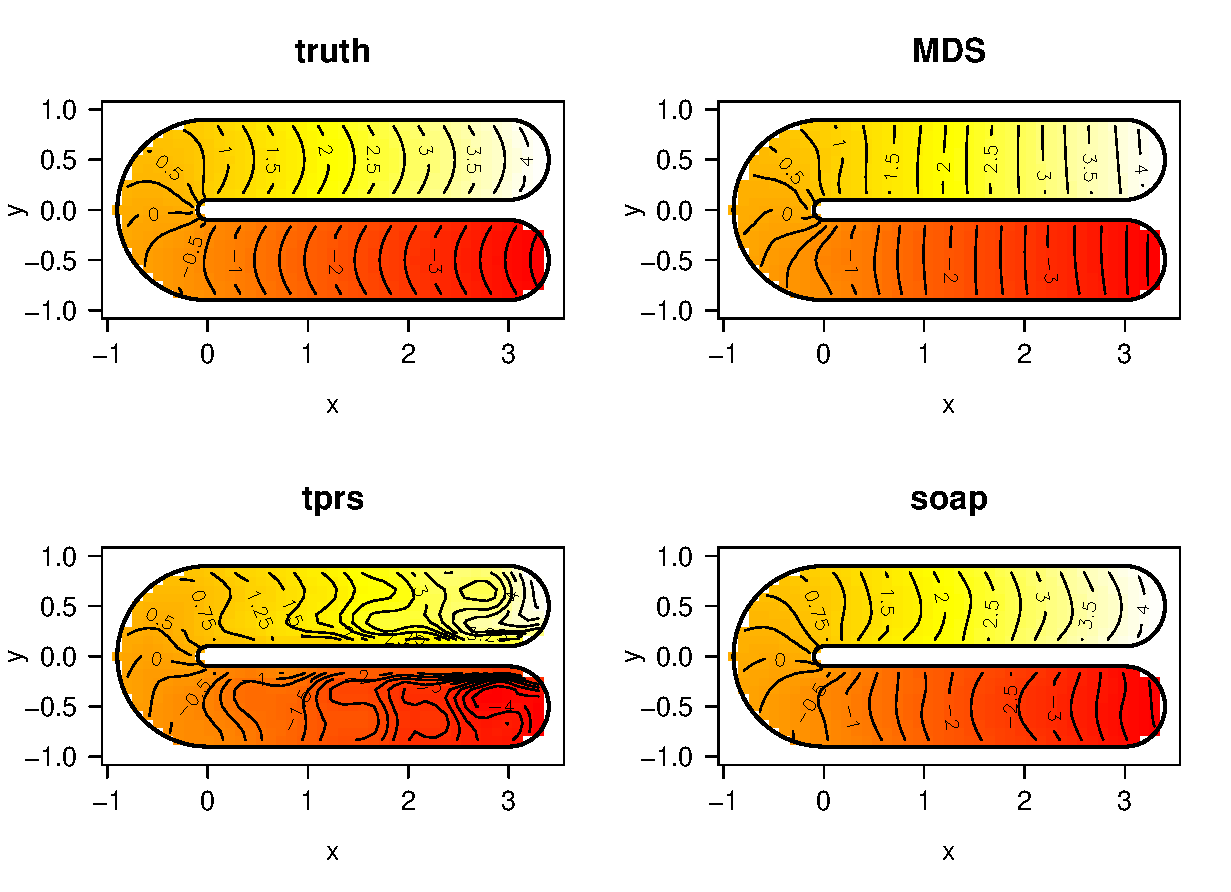
\includegraphics[width=5.5in]{figs/ramsay-mds-smooth-noerr.pdf} \\
\caption{Clockwise from top left: true Ramsay test function, fit given using MDS, thin plate regression spline fit and soap film smooth. Sample size was 250, no noise.}
\label{ramsay-mds-smooth-noerr}
% generate /phd-smoothing/mds/ramsay-smooth-test.R
\end{figure}

Smoothing over these points  in 2D (using a thin plate spline basis) with no error added to a sample of 250 points yields the model shown in \fig{ramsay-mds-smooth-noerr}. Here the plain thin plate fit is has leakage issues, both the MDS fit and the soap film smoother (\cite{soap}) do not exhibit leakage. Looking at the mean squared error we see that [[fill this in]].

%> ramsay_smooth_test(noise.level=0.05)
%$mds
%[1] 0.00251955
%$tprs
%[1] 0.06459767
%$soap
%[1] 0.001559180
%> ramsay_smooth_test(noise.level=0.05)
%$mds
%[1] 0.002114538
%$tprs
%[1] 0.0872122
%$soap
%[1] 0.001085477

%> ramsay_smooth_test(noise.level=0)
%$mds
%[1] 0.001612497
%$tprs
%[1] 0.1072480
%$soap
%[1] 0.000800164
%> ramsay_smooth_test(noise.level=0)
%$mds
%[1] 0.001751240
%$tprs
%[1] 0.0753973
%$soap
%[1] 0.0007361255




% Ramsay MDS smooth fit (with noise)



\subsection{Domain with peninsulae}

\Fig{wt2dia} shows another domain which is more complicated than the horseshoe. The region has peninsulae which will cause similar problems to those found in the horseshoe but additionally has other features. This domain is intended to replicate some of the problems that come about when dealing with coastlines.

An additional complication is that the peninsulae become smaller from left to right, thus the first couple of eigenvectors will be used to explain the variation along the bigger peninsulae and across the baseline. Indeed, we can see this in \fig{wt2dia}.

% plot of points in wt2.
\begin{figure}
\centering
% trim order l b r t
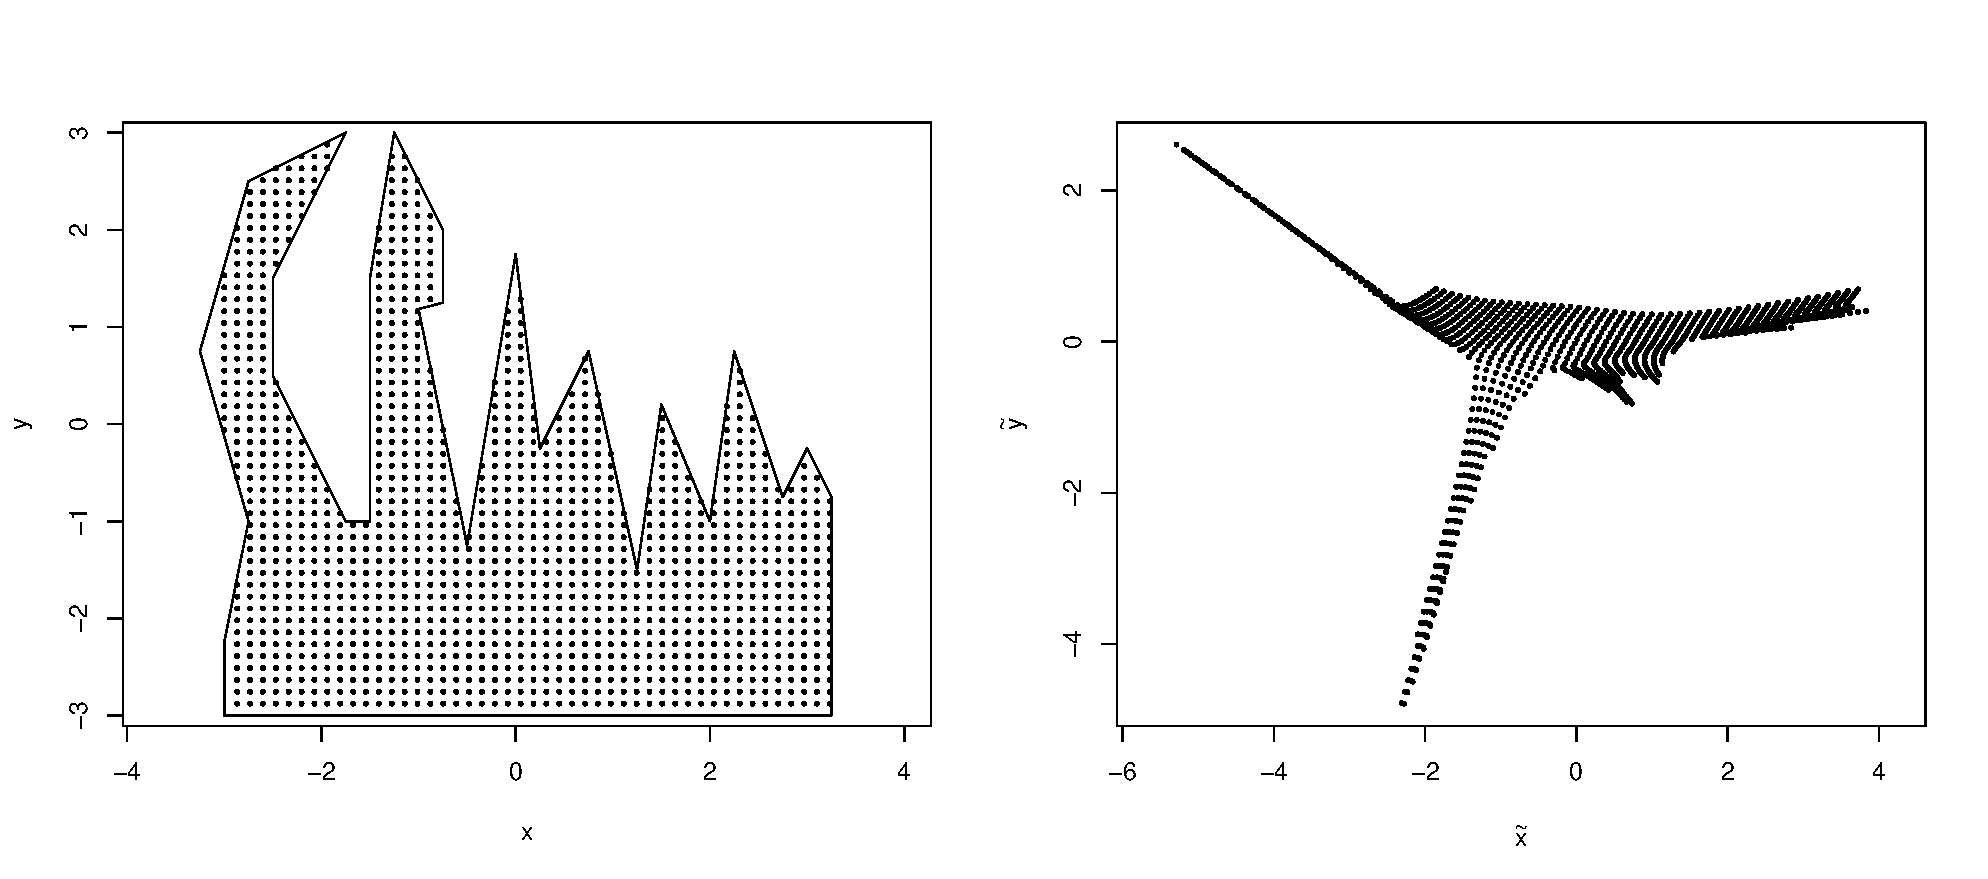
\includegraphics[width=6in]{figs/wt2-mds.pdf}\\
\caption{A domain with many peninsulae (left), and its MDS representation in two dimensions (right) for 1253 points in the domain.}
\label{wt2dia}
\end{figure}

Taking the MDS configuration and smoothing over it (again using a thin plate basis,) we obtain the fits shown in the top right panels of \fig{wt2-mds-smooth-noerr} (with no error) and \fig{wt2-mds-smooth-err} (with $\sigma=0.05$) when the sample size is 250. We again see that the leakage in the thin plate fit is not apparent in the MDS fit. However, although the main features of the true surface are captured, the model does not pick up the features on the right side of the domain. It seems that this is because of the compacting of these features by the MDS routine, as can be seen in \fig{wt2dia}. In both cases the mean squared error for the MDS fit is higher than (but of the same order as) that of the thin plate spline, but without the problem of leakage.

%noise=0
%$mses$mds
%[1] 0.1074302
%$mses$tprs
%[1] 0.06047138
%$mses$soap
%[1] 0.0346587
%
%noise=0.05
%$mses
%$mses$mds
%[1] 0.1164078
%$mses$tprs
%[1] 0.1006808
%$mses$soap
%[1] 0.02077468

% wt2 MDS smooth, no error 
\begin{figure}
\centering
% trim order l b r t
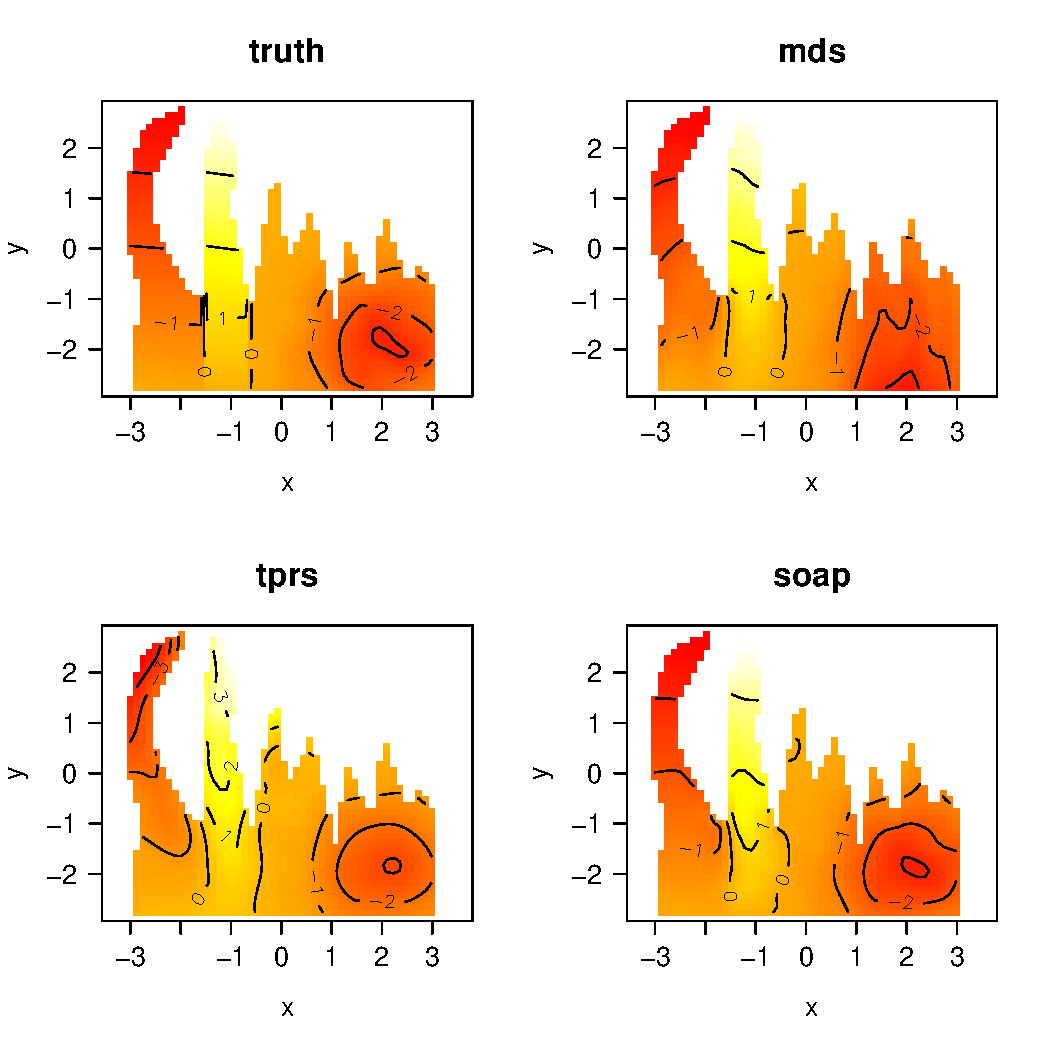
\includegraphics[width=6in]{figs/wt2-mds-smooth-noerr.pdf}\\
\caption{Clockwise from top left: true Ramsay test function, fit given using MDS, thin plate regression spline fit and soap film smooth. Sample size was 250, no noise added to the data.}
\label{wt2-mds-smooth-noerr}
\end{figure}


% wt2 MDS smooth, error 
\begin{figure}
\centering
% trim order l b r t
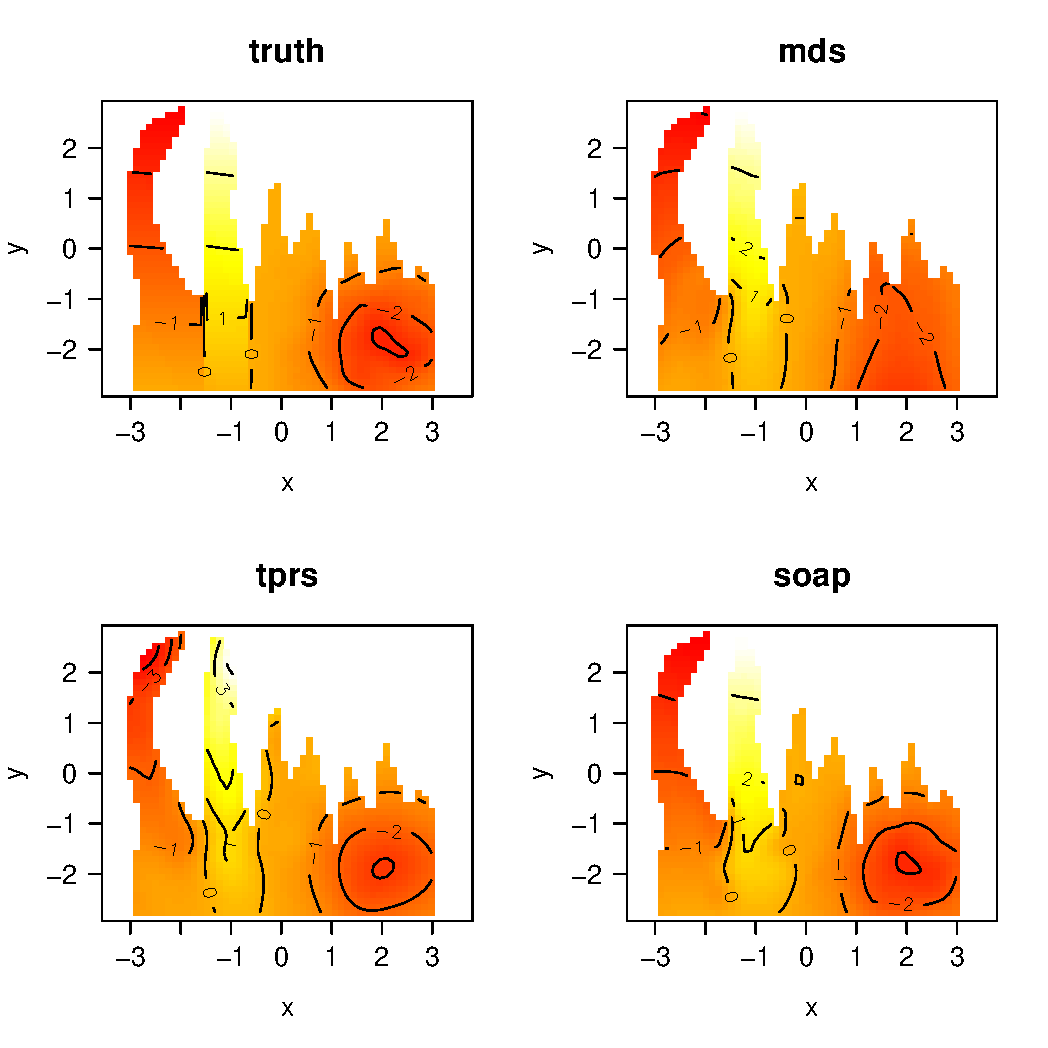
\includegraphics[width=6in]{figs/wt2-mds-smooth-err.pdf}\\
\caption{Clockwise from top left: true Ramsay test function, fit given using MDS, thin plate regression spline fit and soap film smooth. Sample size was 250, noise set at $\sigma^2=0.05$.}
\label{wt2-mds-smooth-err}
\end{figure}

We can see why the fit is capturing the leakage but failing on the right side of the domain by looking at the raw fit on the transformed domain (as produced by \texttt{vis.gam} in \texttt{mgcv} with the \texttt{too.far} option set to 0.04.) \Fig{wt2-visgam} shows the surface with the data plotted ontop. Here we see that there is quite a lot of information in the right side of the domain, but it is being supressed by the penalty (there are plenty of samples here but \fig{wt2-mds-smooth-err} and \fig{wt2-mds-smooth-noerr} do not show much detail in that area.)

% wt2 vis.gam output 
\begin{figure}
\centering
% trim order l b r t
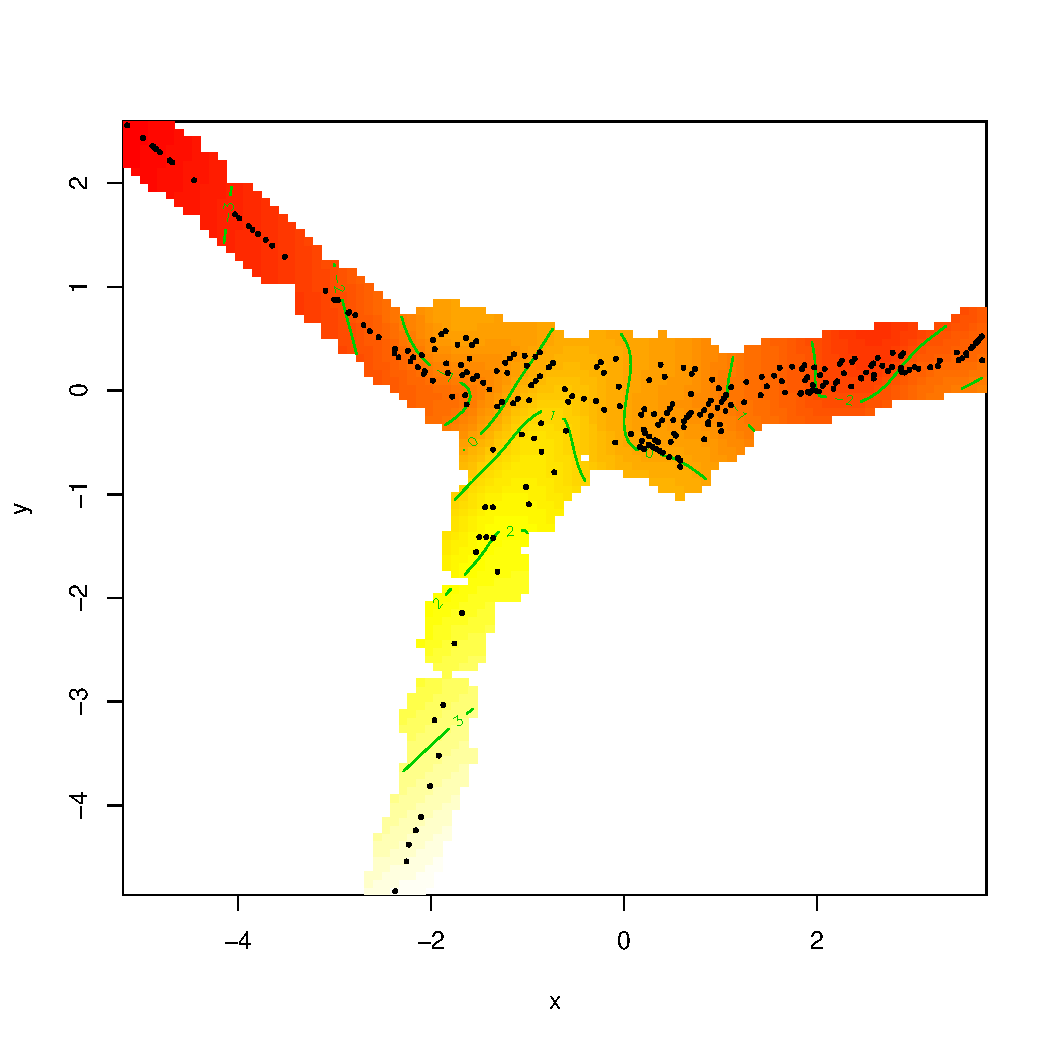
\includegraphics[width=4in]{figs/wt2-visgam.pdf}\\
\caption{Raw fit of the model in the transformed space for the domain with multiple peninsulae. Points lie on the sample data locations.}
\label{wt2-visgam}
\end{figure}

Further evidence to this can be seen if the mean squared error is calculated based on only those points with $x$ coordinates less than 0. In that case the MSE for the MDS fit is about half that of the plain thin plate fit (rather than larger) and is about the same order as the soap film smoother.

So, it would seem that there needs to be some adjustment of the penalty in order to account for the compacting of space by the mapping.

\section{Conclusions}

Although these results are encouraging, the inability of the smooth to capture the features in the right side of the domain is disappointing. Proposed further work is to follow the lead from \cite{wood2000}, which shows that given some transform of a variable, $y$ say, such that $y_i^\prime=y_i/k$, then $f(x,y^\prime k)$ will give the same fit as $f(x,y)$ (ie. the fit will be the same under the new coordinates) but the penalty will change to:

\begin{equation}
\int\int_\Omega \Big( \frac{\partial^2 f}{\partial x^2} \Big) + 2k\Big( \frac{\partial^2 f}{\partial x \partial y} \Big) + k^3\Big( \frac{\partial^2 f}{\partial y^2} \Big) \text{d}x \text{d}y,
\label{adjustedintegral}
\end{equation}

from:

\begin{equation*}
\int\int_\Omega \Big( \frac{\partial^2 f}{\partial x^2} \Big) + 2\Big( \frac{\partial^2 f}{\partial x \partial y} \Big) + \Big( \frac{\partial^2 f}{\partial y^2} \Big) \text{d}x \text{d}y.
\end{equation*}

In the case of the MDS, the integral would need to be split over a grid such that each cell captured the distortion in space over the area of the cell. Mathematically, $\Omega$ would be split into a subsets, $\omega_i$ (where $\bigcup_{\forall j} \omega_j = \Omega$) and (\ref{adjustedintegral}) becomes:

\begin{equation}
\sum_{\forall j} \int\int_{\omega_j} l_j^3 \Big( \frac{\partial^2 f}{\partial x^2} \Big) + 2k_jl_j\Big( \frac{\partial^2 f}{\partial x \partial y} \Big) + k_j^3\Big( \frac{\partial^2 f}{\partial y^2} \Big) \text{d}x \text{d}y,
\label{adjustedintegral}
\end{equation}

where $k_j$ is the scaling in the $y$ direction and $l_j$ is the scaling in the $x$ direction for the $j^{\text{th}}$ cell. We assume here that $f(x,y)$ is ``nice''.

Using this penalty may allow for the distortions in space to be taken account of and therefore get around the problem of the details being smoothed over, as seen above. It will be easiest to first build this using a tensor product of $P$-splines, since their penalty is discrete to test its utility and then move on to the thin plate spline penalty.

Speed and landmark.




\bibliographystyle{plainnat}
\bibliography{mds-refs}

\end{document}
